\documentclass[12pt, a4paper]{article}
\usepackage[margin = 1in, top=1.3in]{geometry}
\usepackage[english]{babel}
\usepackage[utf8]{inputenc}
\usepackage{fancyhdr}
\usepackage[fleqn]{amsmath}
\usepackage{mathtools}
\usepackage{tabto}
\usepackage{bm}
\usepackage{graphicx}
\graphicspath{{./images/}}
\usepackage[font=small,labelfont=bf]{caption}
 
\pagestyle{fancy}
\fancyhf{}
\rhead{\small{Shaan Ul Haque(180070053)\\ Samarth Singh (180050090) \\ Niraj Mahajan (180050069)}}
\lhead{CS-663 Assignment-3 : Question 3}
\rfoot{Page 1.\thepage}
 
\begin{document}
\vspace*{-22pt}
\section*{Question 3}
\subsection*{3.1 : Approach to the problem}
\quad In this section, I have summarised the basic approach to the problem that I have used, along with the assumptions that I made. The essence of the problem is to separate the foreground from the background, given that the foreground is distinctively separable from the background. \\
\null\quad Our basic approach is to generate bounding edges on the foreground using Canny's Edge Detector, and to flood fill the foreground within the detected edges. Then generate a radius matrix, (which has the smallest distance from a pixel to the foreground), and use this to perform spatially varying blurring. Here I have assumed that the foreground will be in the spatial centre of the image. Basically, we need a coordinate of our foreground to perform flood-filling. In a way, this is automatic, as our phone cameras also have a feature where we can tap on a person (in the camera app) and the camera focusses on him/her. The only input/effort that is need from us is to fine une the parameters of Canny Edge Detection. Another assumption that I made is that the foreground is a continuous blob of pixels. (More on this in Section 3.2)

\subsection*{3.2 : Forground Mask Generation}
\quad\quad In this section, the exact algorithm to generate a foreground mask, given an input image is mentioned in detail, and the motivation behind all the sub parts and steps is justified.
\subsubsection*{3.2.1 Edge Detection}
\quad\quad We perform a modified Canny Edge Detection of the input image, with the modification being, we do not apply Non Maximal Suppression. The catch here is that when we try to flood fill the image, even a tiny gap of a single pixel will flood the entire image. Hence we do away with Non Maximal Suppression, but at the cost of more noisy edges being introduced in the background. \\
Here are the fine tuned parameters that I used for both the images:
\vspace*{-8pt}
\begin{itemize}
\item \textbf{Flower: } $\sigma_{g}$ = 0.7
\item \textbf{Flower: } threshold$_{hi}$ =  0.315
\item \textbf{Flower: } threshold$_{lo}$ =  0.18
\item \textbf{Bird: } $\sigma_{g}$ = 0.7
\item \textbf{Bird: } threshold$_{hi}$ =  0.43
\item \textbf{Bird: } threshold$_{lo}$ =  0.25
\end{itemize}

\subsubsection*{3.2.2 Performing Flood Filling on the foreground mask}
\quad\quad Now that we have obtained the edge boundary of the input image, we want to perform a flood fill, so that we isolate the foreground from the background. It is necessary to ensure that the edges of foreground are closed, hence we keep the threshold$_{lo}$ of Canny Hysterisis Thresholding a bit lower than usual. The idea is, some extra noisy edges are acceptable, by the lack of an edge on the foreground isn't. This is, again the same reason why we did not perform Non Maximal Suppression while performing edge detection. We use matlab's $imfill$ function to perform flood filling (as this exploits multi threading of the cpu and is very fast). This flood filling is performed with the centre of the image as an initial point.

\subsubsection*{3.2.3 Removing Noisy Edges and Blobs}
\quad\quad After the flood filling done in Section 3.2.2 we, obtain a noisy mask with many edges in the background, and some unnecessary flood filled blobs that extend to the background. In order to remove these, we perform median filtering on the image with a relatively large window size. Our assumption here is the most of the background will have 0s while most for the foreground will have 1s. So the outliers in the image which do no follow this trend get corrected by performing median filtering. \\
\null\quad\quad Now we have pure and continuous blobs of foreground and background. But we may have multiple blobs. For example, the mask of the flower has two blobs, one that covers the flower, and the other (smaller) that covers a part of a leaf. We need to remove blobs like these. For this we use matlab's inbuilt $bwareafilt$ function, which filters out blobs and preserves the one with the highest area.

\subsubsection*{3.2.3 Reclaiming the trimmed foreground}
\quad\quad When we applied median filtering in section 3.2.2, some part of the foreground was lost, since the median at the peripheral points of the foreground will lie in the background. Note that the flood filling was performed on the foreground mask which is a matrix of logical bits. Hence in order to reclaim this lost/approximated area, we perform an operation quite similar to Non Maximal Suppression. 
\begin{itemize}
\item Iterate over all the pixels P in the foreground mask, such that the value assigned to P is 0, ie, background
\item Compute the 8-neighborhood of Pixel P
\item If there exist any pixel that is assigned 1 in this neigh	
\end{itemize}
We go over the foreground mask, and for every pixel that is assigned 0 (ie, background), we check its 8-neighborhood. If there lies a pixel that is assigned 1 (ie foreground) in its neighborhood, we set this pixel to 1. 
\begin{flushright}
...We finally have our foreground mask!
\end{flushright} 
\newpage
\subsubsection*{3.2.3 Results of the foreground generation algorithm}
The following are the results obtained on \textbf{flower.jpg} and \textbf{bird.jpg}.
\vspace*{-15pt}
\begin{figure}[h!]
    \centering
    \renewcommand{\thefigure}{3.1(a)}
    \begin{minipage}[c][1\width]{0.3\textwidth}
    	\hspace*{-0.5in}
    	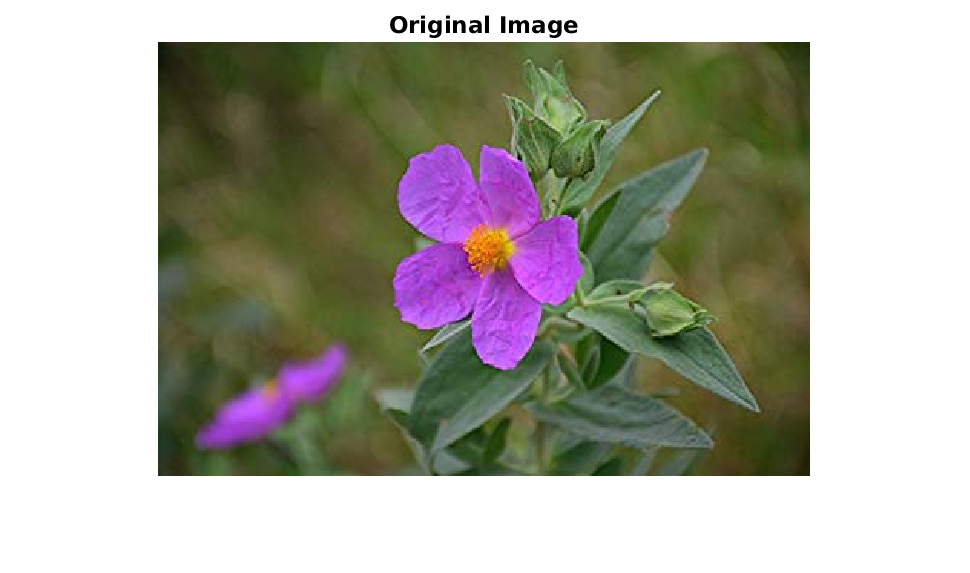
\includegraphics[width=1.44\textwidth]{flower_original.png}
    	\null\vspace*{-28pt}
    	\caption{Original}
	    \label{fig:3.1(a)}
    \end{minipage} \\
    \renewcommand{\thefigure}{3.1(b)}
    \begin{minipage}[c][1\width]{0.3\textwidth}
    	\hspace*{-1in}
    	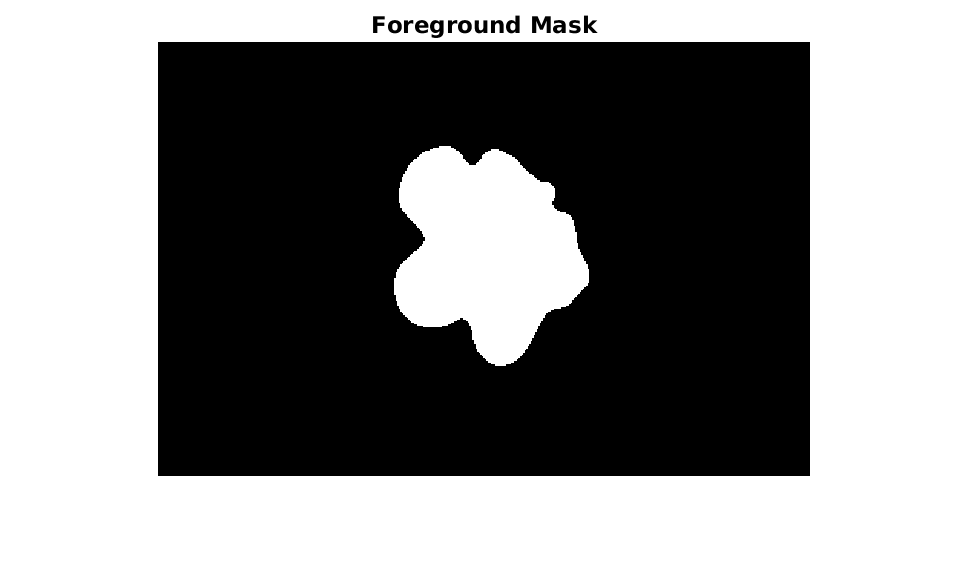
\includegraphics[width=1.5\textwidth]{flower_mask.png}
    	\null\vspace*{-28pt}
    	\caption{Mask}
	    \label{fig:3.1(b)}
    \end{minipage}
    \renewcommand{\thefigure}{3.1(c)}
    \begin{minipage}[c][1\width]{0.3\textwidth}
    	\hspace*{-0.5in}
    	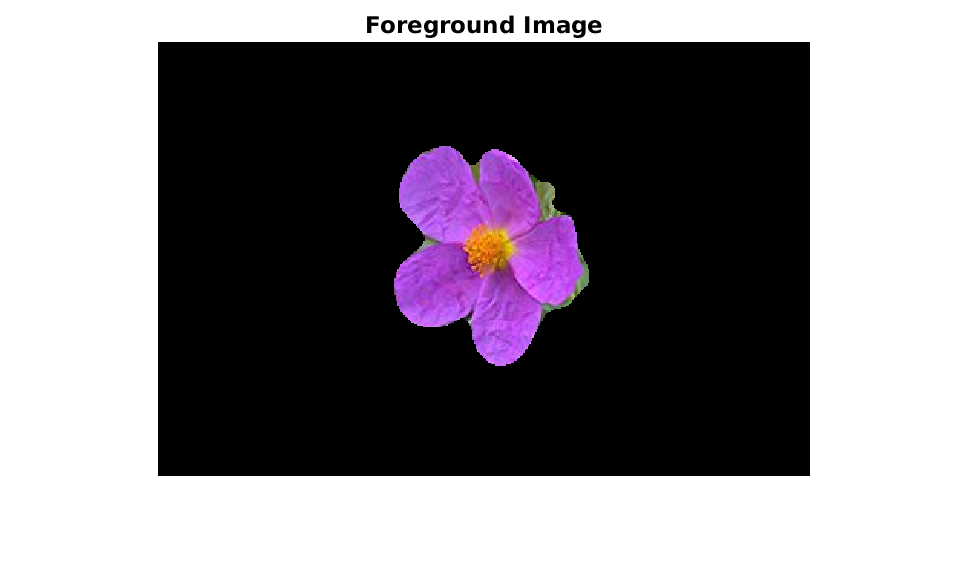
\includegraphics[width=1.5\textwidth]{flower_foreground.png}
    	\null\vspace*{-28pt}
    	\caption{Foreground}
	    \label{fig:3.1(c)}
    \end{minipage}
    \renewcommand{\thefigure}{3.1(d)}
    \begin{minipage}[c][1\width]{0.3\textwidth}
    	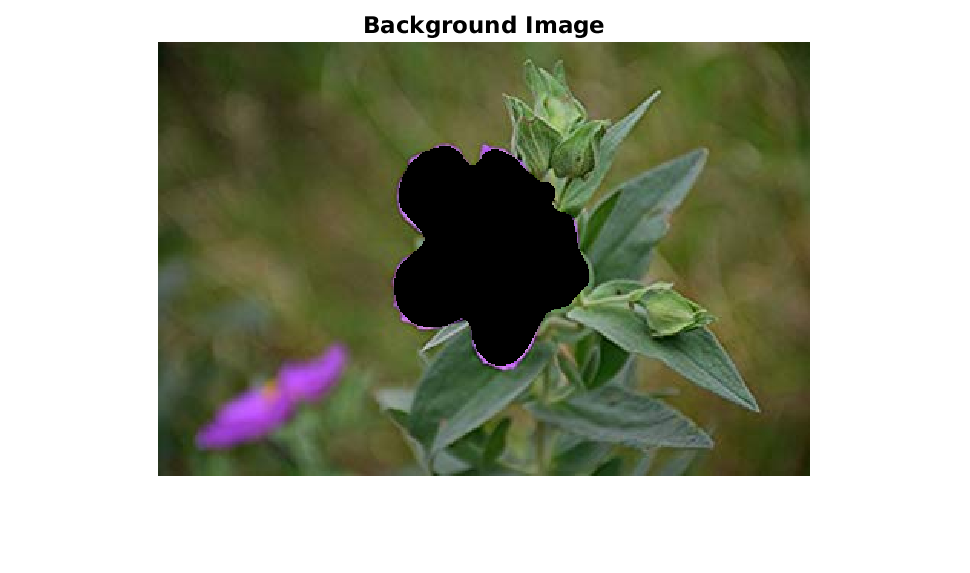
\includegraphics[width=1.5\textwidth]{flower_background.png}
    	\null\vspace*{-28pt}
    	\caption{Backgr.}
	    \label{fig:3.1(d)}
    \end{minipage}
	\\
    \renewcommand{\thefigure}{3.2(a)}
    \begin{minipage}[c][1\width]{0.3\textwidth}
    	\hspace*{-0.5in}
    	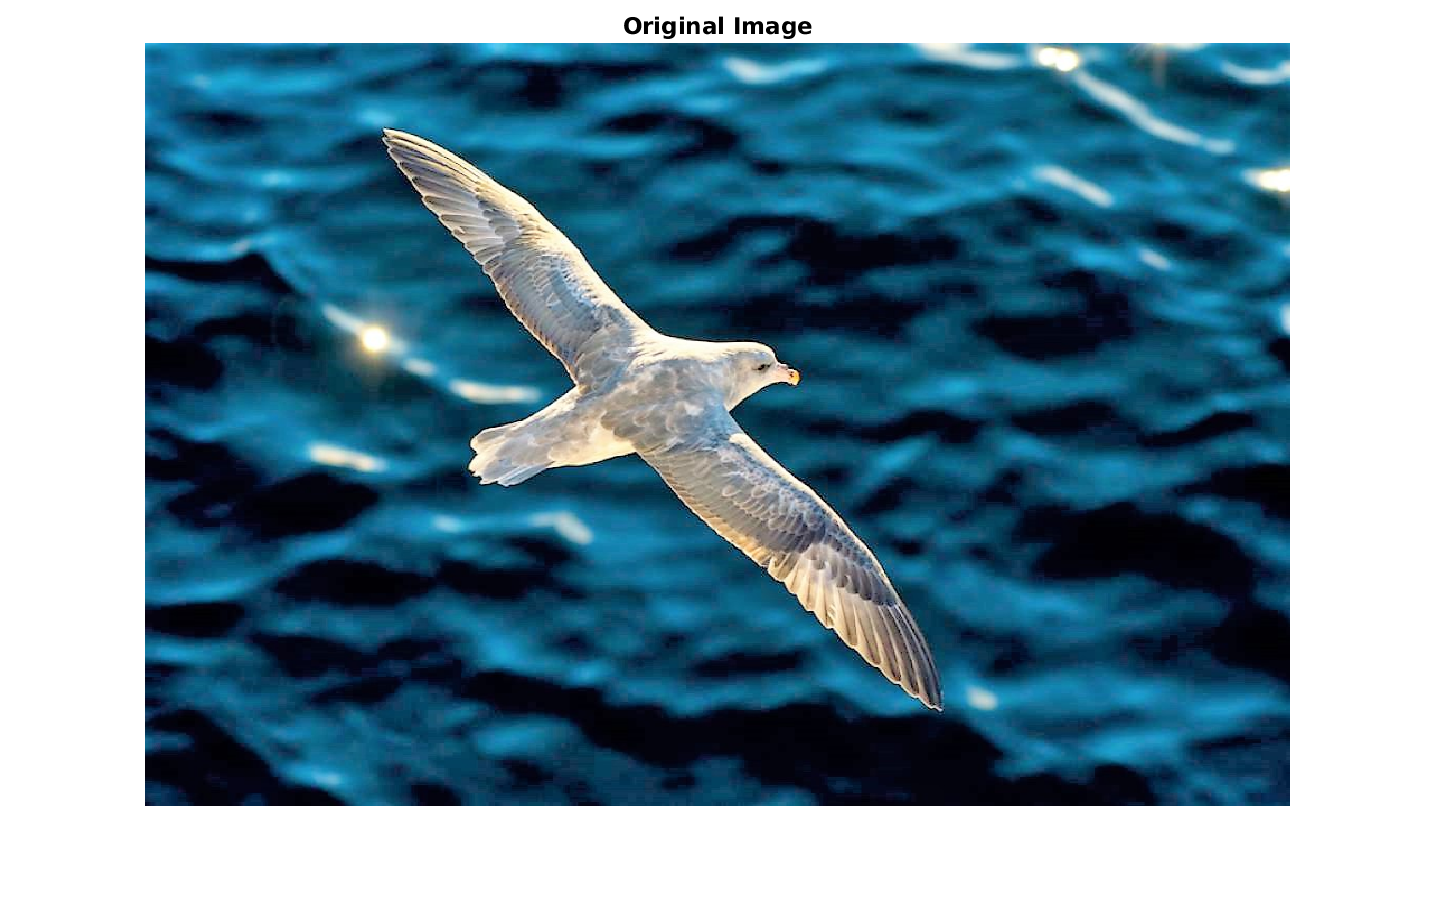
\includegraphics[width=1.44\textwidth]{bird_original.png}
    	\null\vspace*{-28pt}
    	\caption{Original}
	    \label{fig:3.2(a)}
    \end{minipage} \\
    \renewcommand{\thefigure}{3.2(b)}
    \begin{minipage}[c][1\width]{0.3\textwidth}
    	\hspace*{-1in}
    	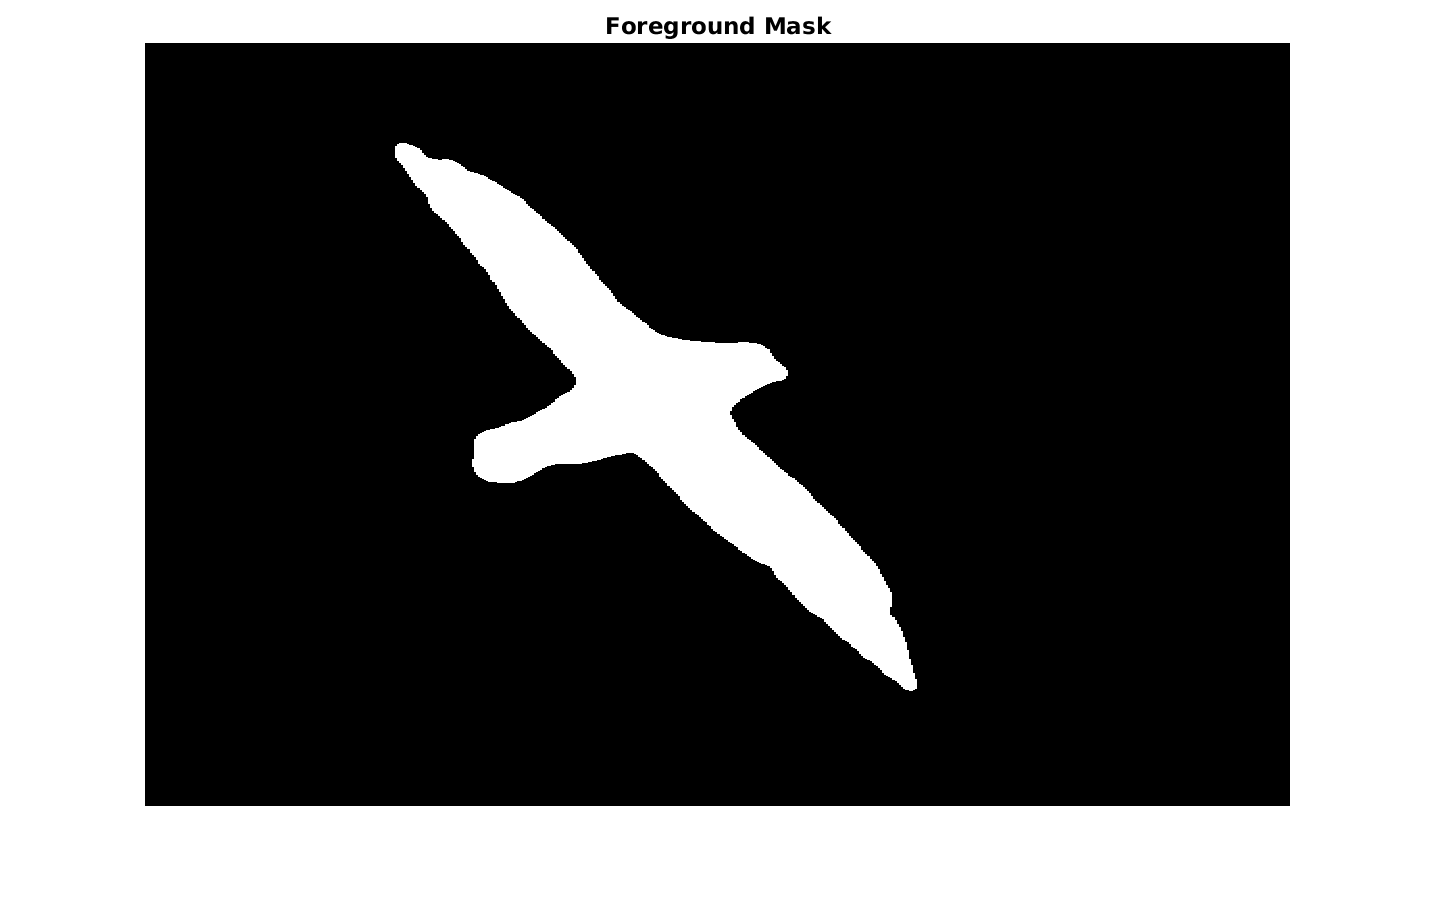
\includegraphics[width=1.5\textwidth]{bird_mask.png}
    	\null\vspace*{-28pt}
    	\caption{Mask}
	    \label{fig:3.2(b)}
    \end{minipage}
    \renewcommand{\thefigure}{3.2(c)}
    \begin{minipage}[c][1\width]{0.3\textwidth}
    	\hspace*{-0.5in}
    	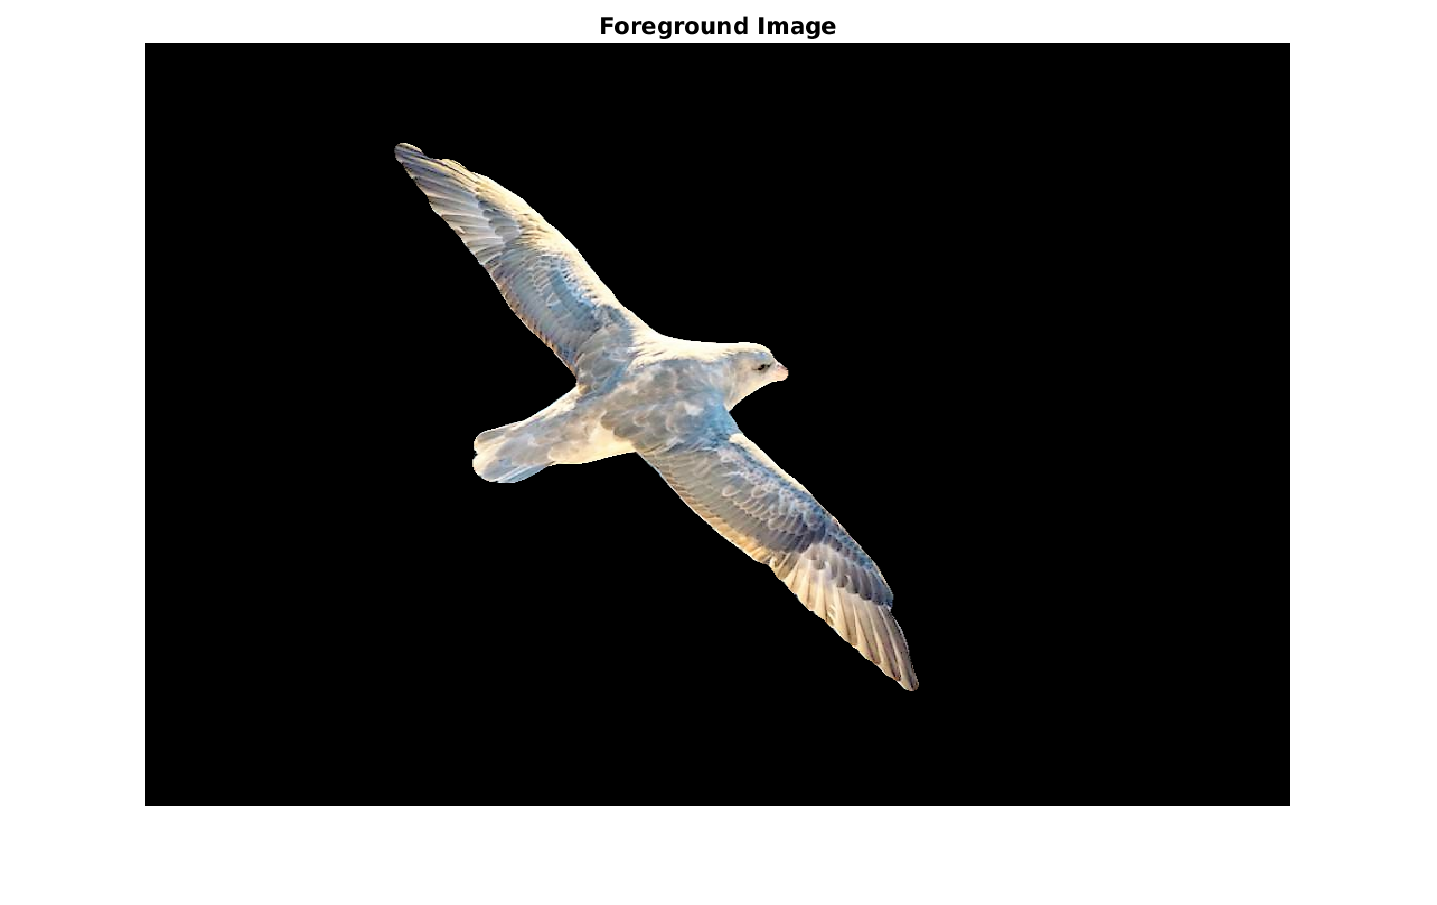
\includegraphics[width=1.5\textwidth]{bird_foreground.png}
    	\null\vspace*{-28pt}
    	\caption{Foreground}
	    \label{fig:3.2(c)}
    \end{minipage}
    \renewcommand{\thefigure}{3.2(d)}
    \begin{minipage}[c][1\width]{0.3\textwidth}
    	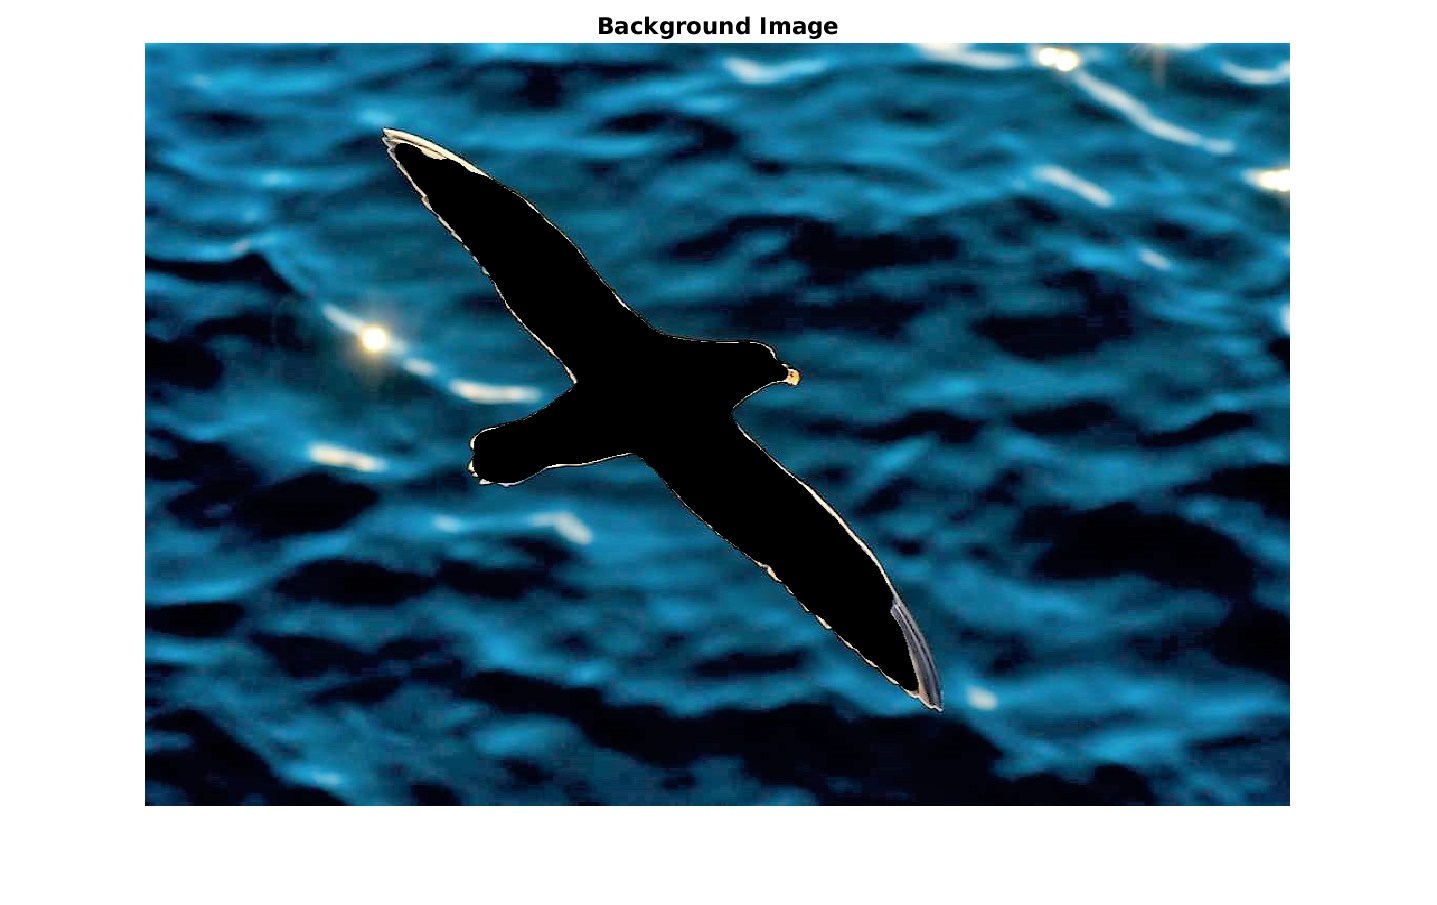
\includegraphics[width=1.5\textwidth]{bird_background.png}
    	\null\vspace*{-28pt}
    	\caption{Backgr.}
	    \label{fig:3.2(d)}
    \end{minipage}
\end{figure}
\newpage
\subsection*{3.3 : Generating a Spatially Varying Kernel}
\quad\quad Using the foreground mask that we obtained in Section 3.2, we now need to obtain a radii matrix \textbf{R} $= [\;r_{ij}\;]$ such that $r_{i,j}$ at any pixel location i,j is the minimum distance from this pixel to any foreground pixel. We also need to cap these radii at a cutoff value (say $\alpha$), where $\alpha_{flower} = 20$ and $\alpha_{bird} = 40$. 
\vspace*{-15pt}
\begin{figure}[h!]
    \centering
    \renewcommand{\thefigure}{3.3(a)}
    \begin{minipage}[c][1\width]{0.45\textwidth}
    	\hspace*{-0.5in}
    	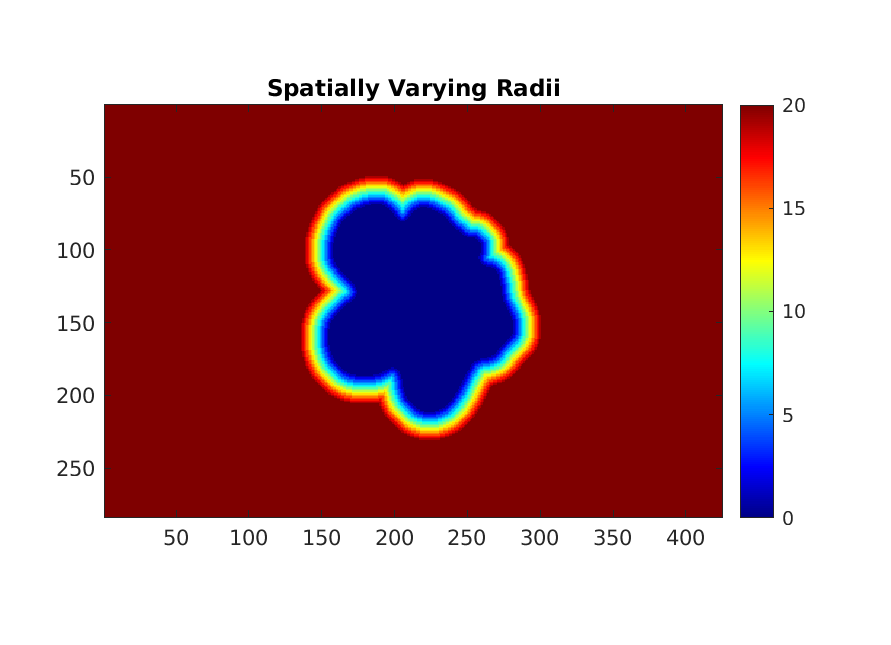
\includegraphics[width=1.24\textwidth]{flower_radii.png}
    	\null\vspace*{-28pt}
    	\caption{Flower Radii}
	    \label{fig:3.3(a)}
    \end{minipage}
        \renewcommand{\thefigure}{3.3(b)}
    \begin{minipage}[c][1\width]{0.45\textwidth}
    	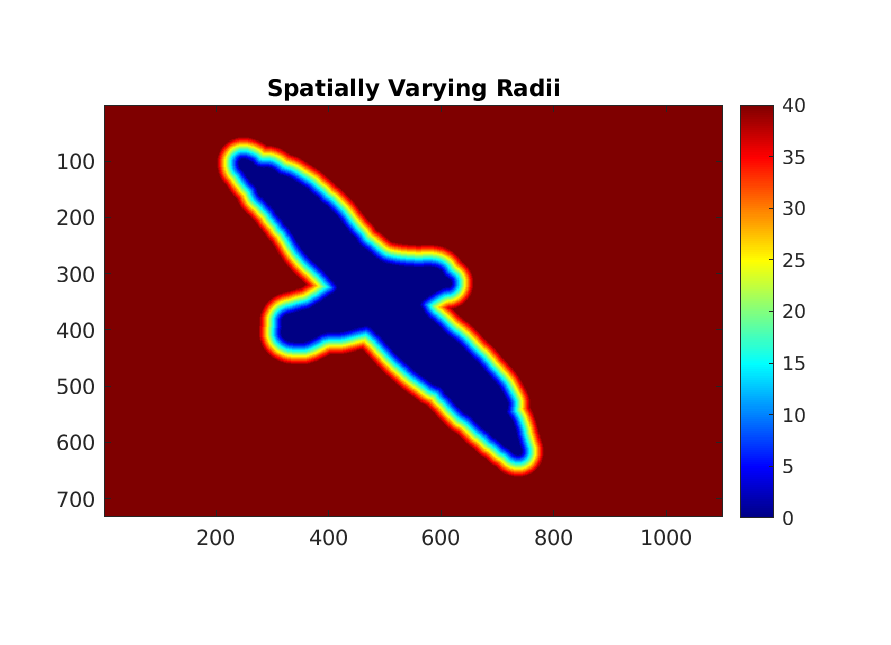
\includegraphics[width=1.24\textwidth]{bird_radii.png}
    	\null\vspace*{-28pt}
    	\caption{Bird Radii}
	    \label{fig:3.3(b)}
    \end{minipage}
\end{figure}
\subsection*{3.4 : Generating Circular Kernel Filters}
In order to perform background blurring, we need circular filters (of varying radius, of course). The corresponding filters at different radii, for flower.jpg and bird.jpg respectively are displayed below.
\begin{figure}[h!]
    \centering
    \begin{minipage}[c][1\width]{0.19\textwidth}
	    \hspace*{-14pt}
    	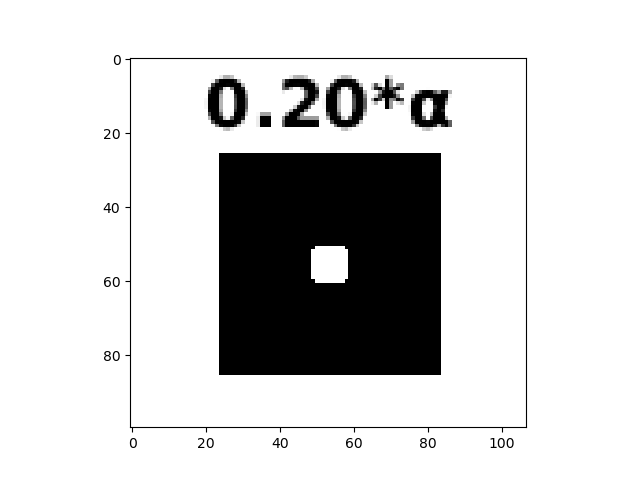
\includegraphics[width=1.24\textwidth]{flower_kernel_0.20_cropped.png}
	    \label{fig:3.4(a)}
    \end{minipage}
    \begin{minipage}[c][1\width]{0.19\textwidth}
        \hspace*{-14pt}
    	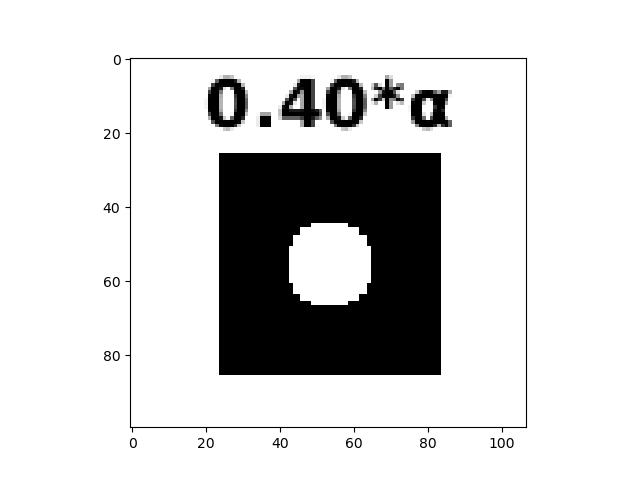
\includegraphics[width=1.24\textwidth]{flower_kernel_0.40_cropped.png}
	    \label{fig:3.4(a)}
    \end{minipage}
\renewcommand{\thefigure}{: flower}
    \begin{minipage}[c][1\width]{0.19\textwidth}
        \hspace*{-14pt}
    	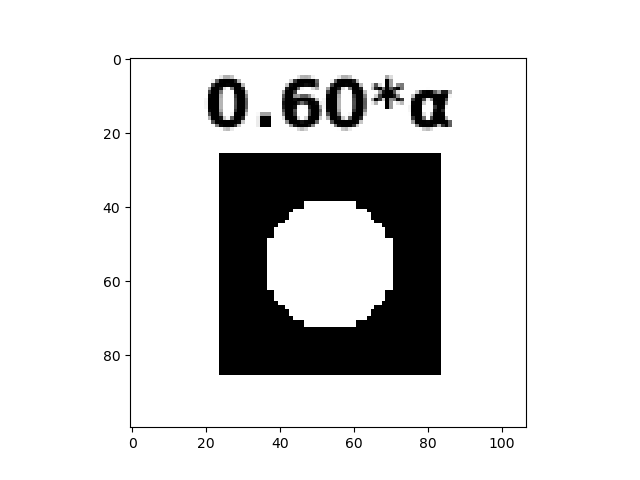
\includegraphics[width=1.24\textwidth]{flower_kernel_0.60_cropped.png}
	    \label{fig:3.4(a)}
	    \vspace*{-23pt}
	    \caption{}
    \end{minipage}
    \begin{minipage}[c][1\width]{0.19\textwidth}
        \hspace*{-14pt}
    	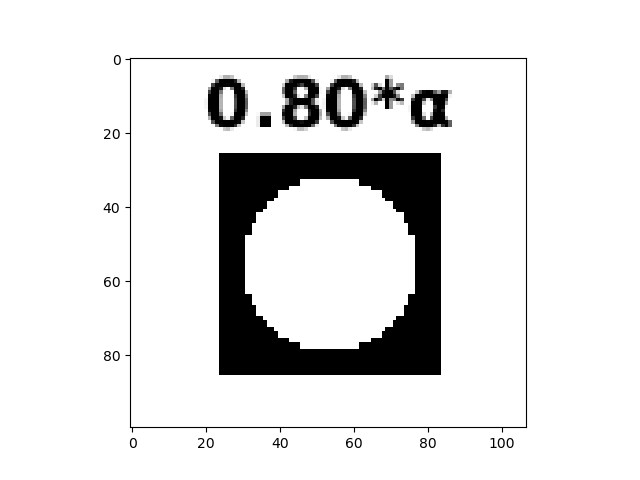
\includegraphics[width=1.24\textwidth]{flower_kernel_0.80_cropped.png}
	    \label{fig:3.4(a)}
    \end{minipage}
    \begin{minipage}[c][1\width]{0.19\textwidth}
        \hspace*{-14pt}
    	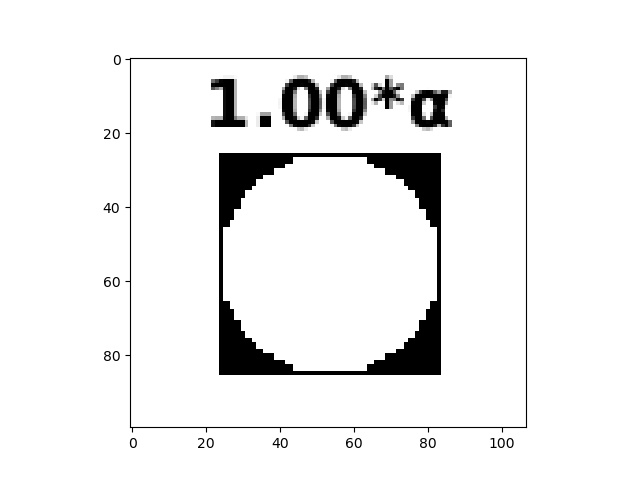
\includegraphics[width=1.24\textwidth]{flower_kernel_1.00_cropped.png}
	    \label{fig:3.4(a)}
    \end{minipage}
\end{figure}

\begin{figure}[h!]
    \centering
    \begin{minipage}[c][1\width]{0.19\textwidth}
    	\hspace*{-14pt}
    	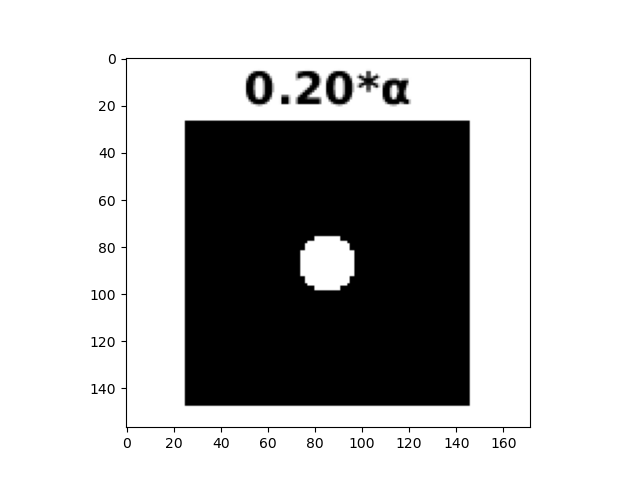
\includegraphics[width=1.24\textwidth]{bird_kernel_0.20_cropped.png}
	    \label{fig:3.5(a)}
    \end{minipage}
    \begin{minipage}[c][1\width]{0.19\textwidth}
    	\hspace*{-14pt}
    	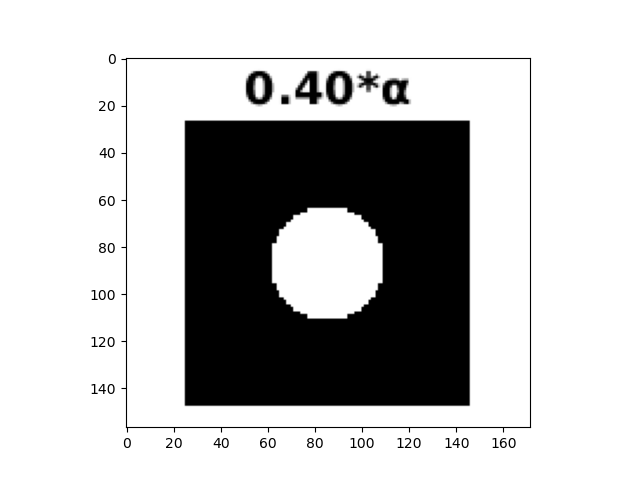
\includegraphics[width=1.24\textwidth]{bird_kernel_0.40_cropped.png}
	    \label{fig:3.5(a)}
    \end{minipage}
\renewcommand{\thefigure}{: bird}
    \begin{minipage}[c][1\width]{0.19\textwidth}
		\hspace*{-14pt}    	
    	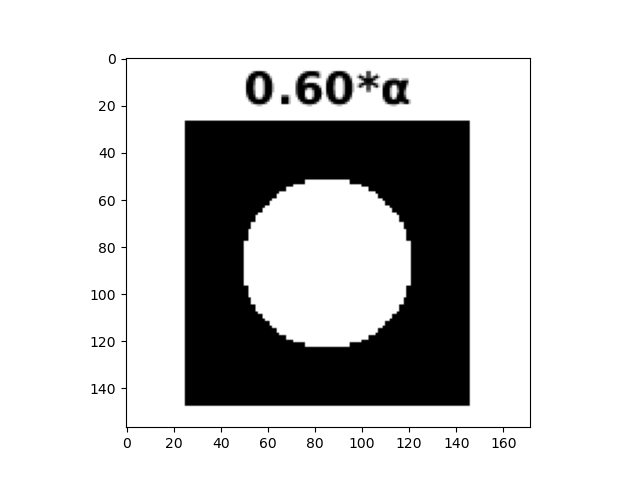
\includegraphics[width=1.24\textwidth]{bird_kernel_0.60_cropped.png}
	    \label{fig:3.5(a)}
	    \vspace*{-23pt}
	    \caption{}
    \end{minipage}
    \begin{minipage}[c][1\width]{0.19\textwidth}
    	\hspace*{-14pt}
    	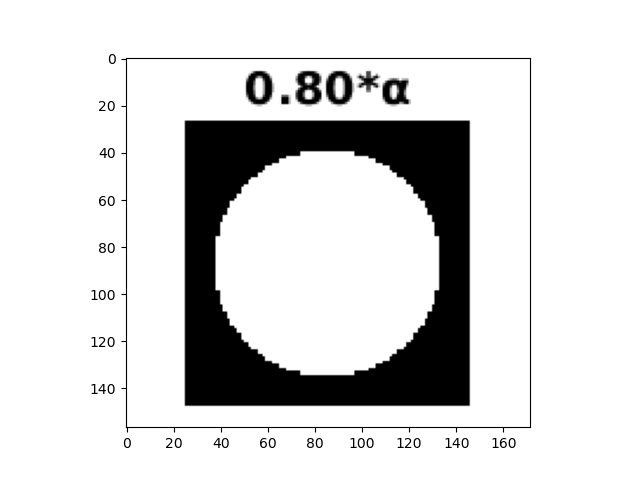
\includegraphics[width=1.24\textwidth]{bird_kernel_0.80_cropped.png}
	    \label{fig:3.5(a)}
    \end{minipage}
    \begin{minipage}[c][1\width]{0.19\textwidth}
    	\hspace*{-14pt}
    	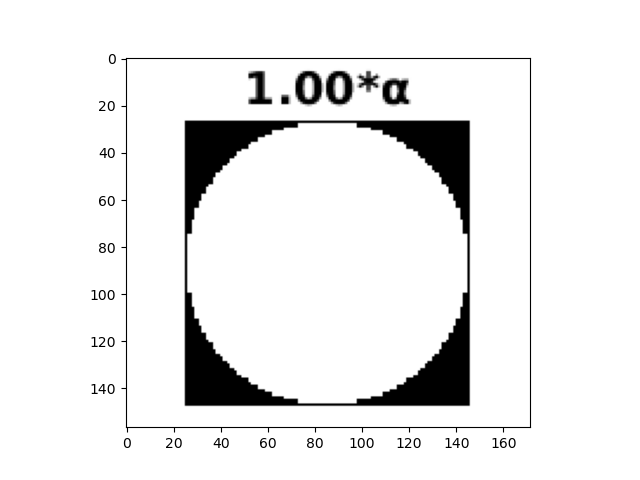
\includegraphics[width=1.24\textwidth]{bird_kernel_1.00_cropped.png}
	    \label{fig:3.5(a)}
    \end{minipage}
\end{figure}
\newpage
\subsection*{3.5 : Final Results}
Using the foreground maks obtained in Section 3.2, the radii matrices obtained in Section 3.3, and the Circular Filters obtained in Section 3.4, we now finally can perform background blurring on our input images. The results are as follows:

\begin{figure}[h!]
    \centering
    \renewcommand{\thefigure}{3.6(a)}
    \begin{minipage}[c][1\width]{0.45\textwidth}
    	\hspace*{-0.5in}
    	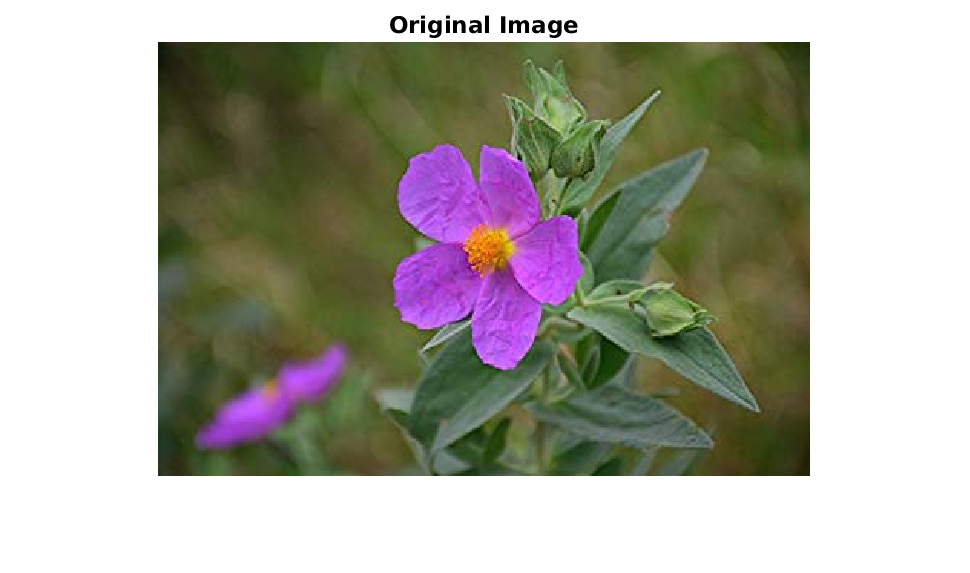
\includegraphics[width=1.24\textwidth]{flower_original.png}
    	\null\vspace*{-28pt}
    	\caption{Original Flower}
	    \label{fig:3.6(a)}
    \end{minipage}
    \renewcommand{\thefigure}{3.6(b)}
    \begin{minipage}[c][1\width]{0.45\textwidth}
    	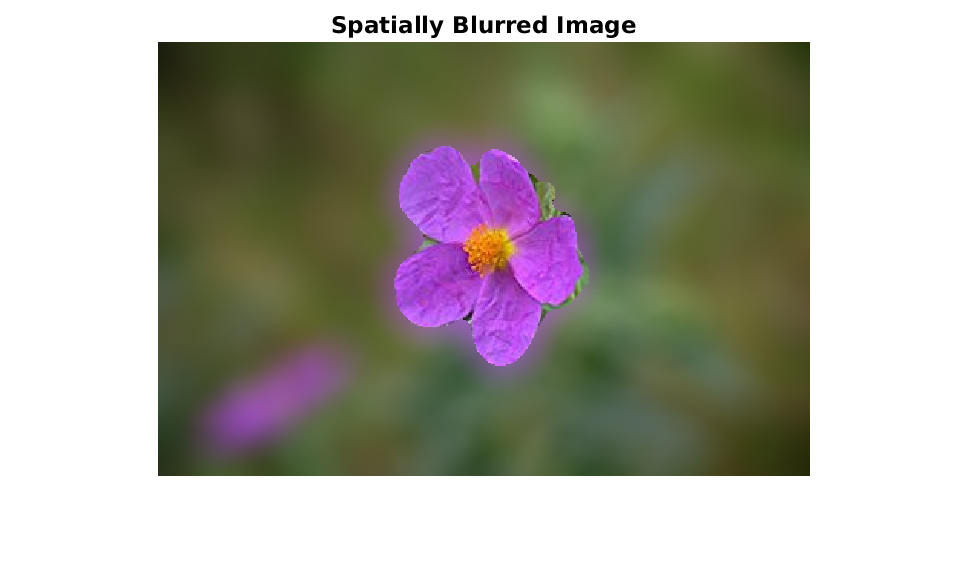
\includegraphics[width=1.24\textwidth]{flower_spatially_blurred.png}
    	\null\vspace*{-28pt}
    	\caption{Blurred Flower}
	    \label{fig:3.6(b)}
    \end{minipage} \\
    \renewcommand{\thefigure}{3.7(a)}
    \begin{minipage}[c][1\width]{0.45\textwidth}
    	\hspace*{-0.5in}
    	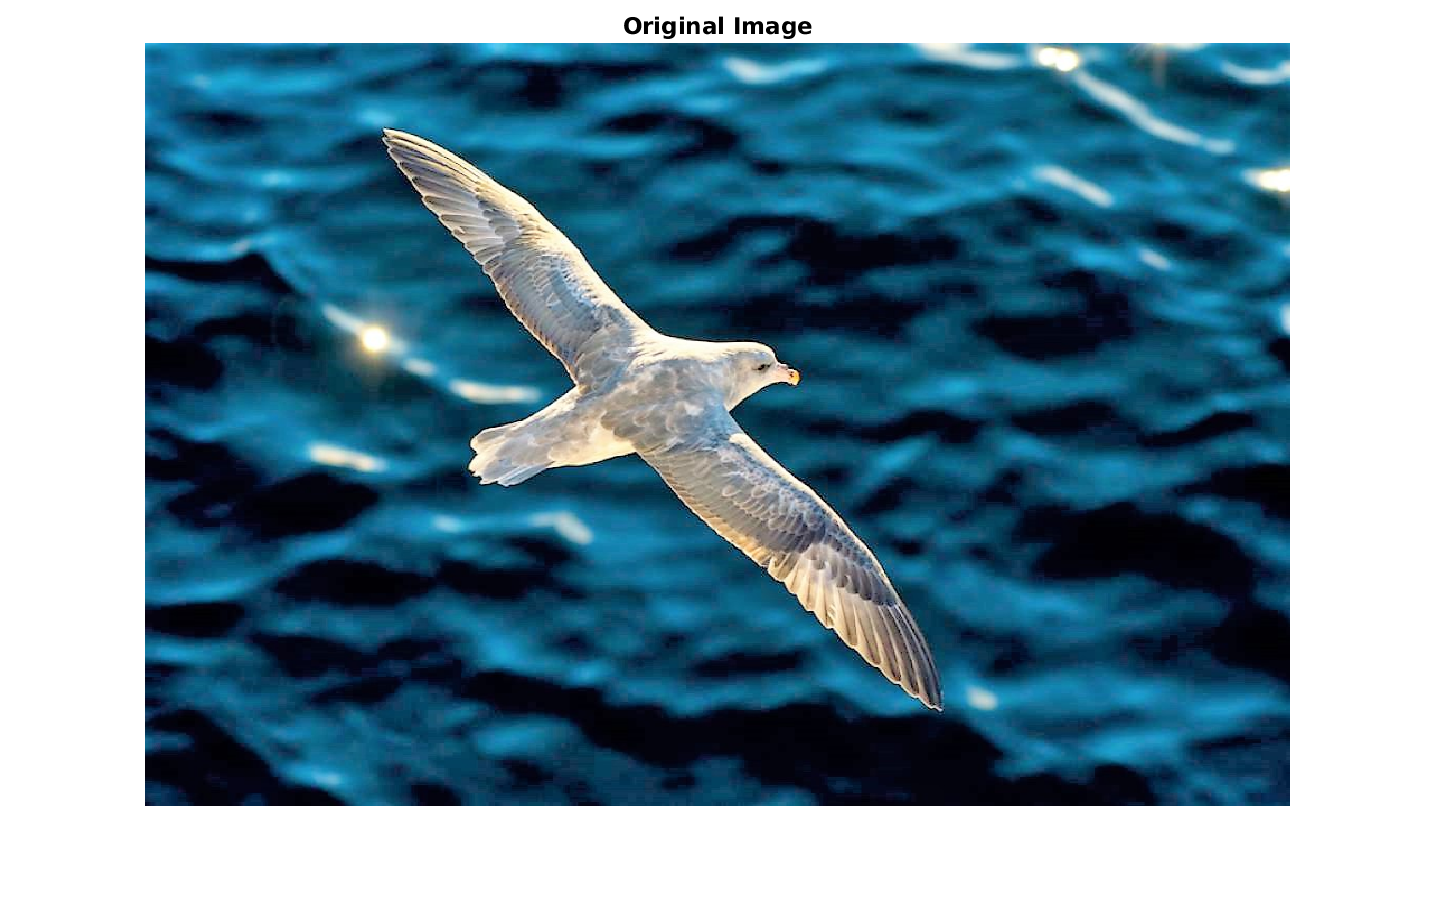
\includegraphics[width=1.24\textwidth]{bird_original.png}
    	\null\vspace*{-28pt}
    	\caption{Original Bird}
	    \label{fig:3.7(a)}
    \end{minipage}
    \renewcommand{\thefigure}{3.7(b)}
    \begin{minipage}[c][1\width]{0.45\textwidth}
    	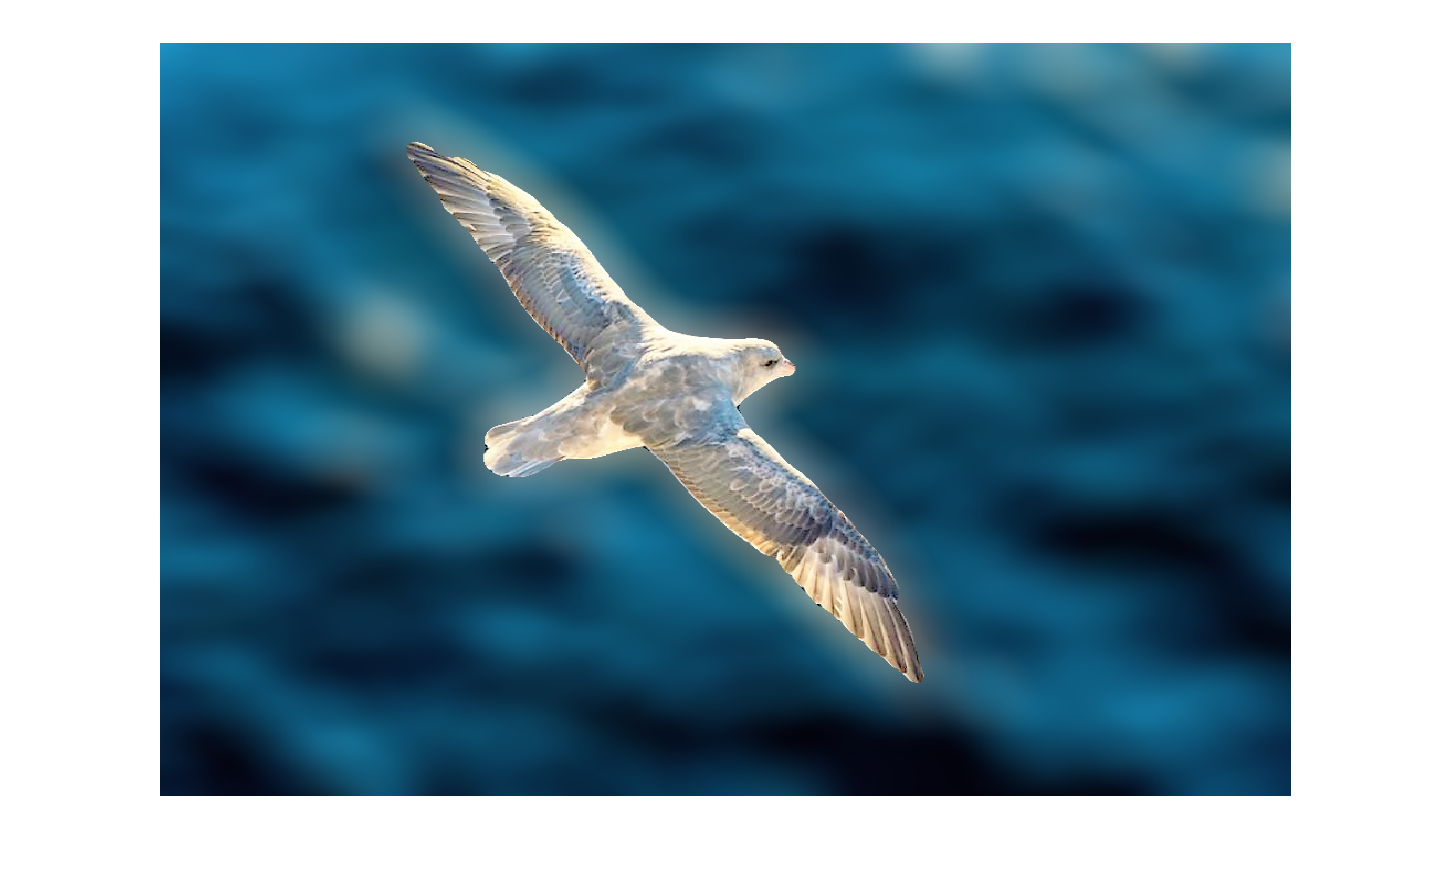
\includegraphics[width=1.24\textwidth]{bird_spatially_blurred.png}
    	\null\vspace*{-28pt}
    	\caption{Blurred Bird}
	    \label{fig:3.7(b)}
    \end{minipage}
\end{figure}
\newpage
\subsection*{3.5 : Usage of Code}
\begin{itemize}
\item The main file \textbf{myMainScript.m} takes about 170 seconds to execute - 6 seconds for flower.png and about 164 seconds for bird.png.
\item The main script has all the parameters that are fine tuned for Canny Edge Detector. There is no other manual human input required, and rest of the process is completely automatic.
\item The main script calls the \textbf{workOnImage.m} function, which appropriately processes each image and saves the outputs as .png
\item The function \textbf{cannyEdgeDetector.m} implements the Canny algorithm, without Non Maximal Suppression (commented out).
\item The function \textbf{getForeground.m} takes as input the original image and the edges obtained, and generates the foreground mask.
\item The function \textbf{getKernel.m} generates a circular filter of a specified radius.
\item The function \textbf{getRadiusMask.m} takes as input the foreground mask, and generates the radii matrix as specified in Section 3.3
\item The function \textbf{mySpatiallyVaryingKernel.m} takes as input the foreground mask, input image, and radii matrix, and performs background blurring on the input image. 
\end{itemize}

\end{document}